\chapter{Implementation}\label{chapter:implementation}

The implementation chapter will provide specific information about the CASA system implemented for the thesis. It will give more attention to the algorithms used in different parts of the architecture and their input parameters. The main goal of the system was to separate monophonic piano music from the background noise by finding an ideal binary mask for the cochleagram. The follow-up experiments will be described later in chapter \ref{chapter:experiments}.\\

It should also be noted, that the implemented system is rather simple, thus it should not be expected to observe source separation of too high quality. The implemented model serves only as an example of a CASA system, and does not aim to separate the sources using the most modern and sophisticated algorithms and approaches.\\

The system is implemented in Python with the help of \textit{numpy} \cite{numpy}, \textit{scipy} \cite{scipy}, \textit{statsmodels} \cite{statsmodels}, \textit{matplotlib} \cite{matplotlib} and \textit{brian2hears} \cite{brian2hears} packages. \textit{Skimage} \cite{scikit-image} and \textit{brian2} \cite{brian2} were used as supporting ones. For evaluation, a simple multi-class classifier was implemented with the help of the \textit{scikit-learn} \cite{scikit-learn} package. The main Python scripts contain functions for different parts of the resulting architecture, and then an example of their usage along with the experiments overview is given in the supporting Jupyter notebooks (see appendix \ref{chapter:medium} for more information).

\section{Cochleagram}

The cochleagram described in section \ref{subsection:casa_peripheral_analysis} was implemented with the help of the \textit{brian2hears}~\cite{brian2hears} package. At the beginning, an array of center frequencies was computed using the ERB-rate scale defined in chapter \ref{section:math_concepts}. In the main example notebook, there were 128 center frequencies uniformly distributed on it between the values of the lowest and the highest fundamental frequencies on the standard piano keyboard (containing 88 keys) -- from $27.5$\,Hz (note $A_0$) to $4.186$\,kHz (note $C_8$).\\

As a next step, a gammatone filterbank was used to split the input into 128 corresponding frequency channels. The filters were implemented as cascades of four IIR filters of order~2 (this corresponds to a set of single gammatone filters of order~4 \cite{brian2hears}). The approximate impulse response was similar to the one defined in equation \ref{equation:gammatone_impulse_response}:
\begin{equation}
	g_{f_c}(t) = t^3\,e^{-2\pi{}bERB(f_c)t}\,\cos(2\pi{}f_c{}t)
\end{equation}
where $b=1.019$ and the ERB function was the same as in equation \ref{equation:ERB_1990} for frequency in Hertz. Finally, a unit-step function was applied to the output along with a cubic root function that helped to better emphasize low amplitudes in the cochleagram. The resulting cochleagrams for C-major and A-major scales are shown on figure \ref{img:cochleagram_example}.\\

\begin{figure}[t]
	\centering
	\begin{subfigure}{0.5\textwidth}
		\centering
		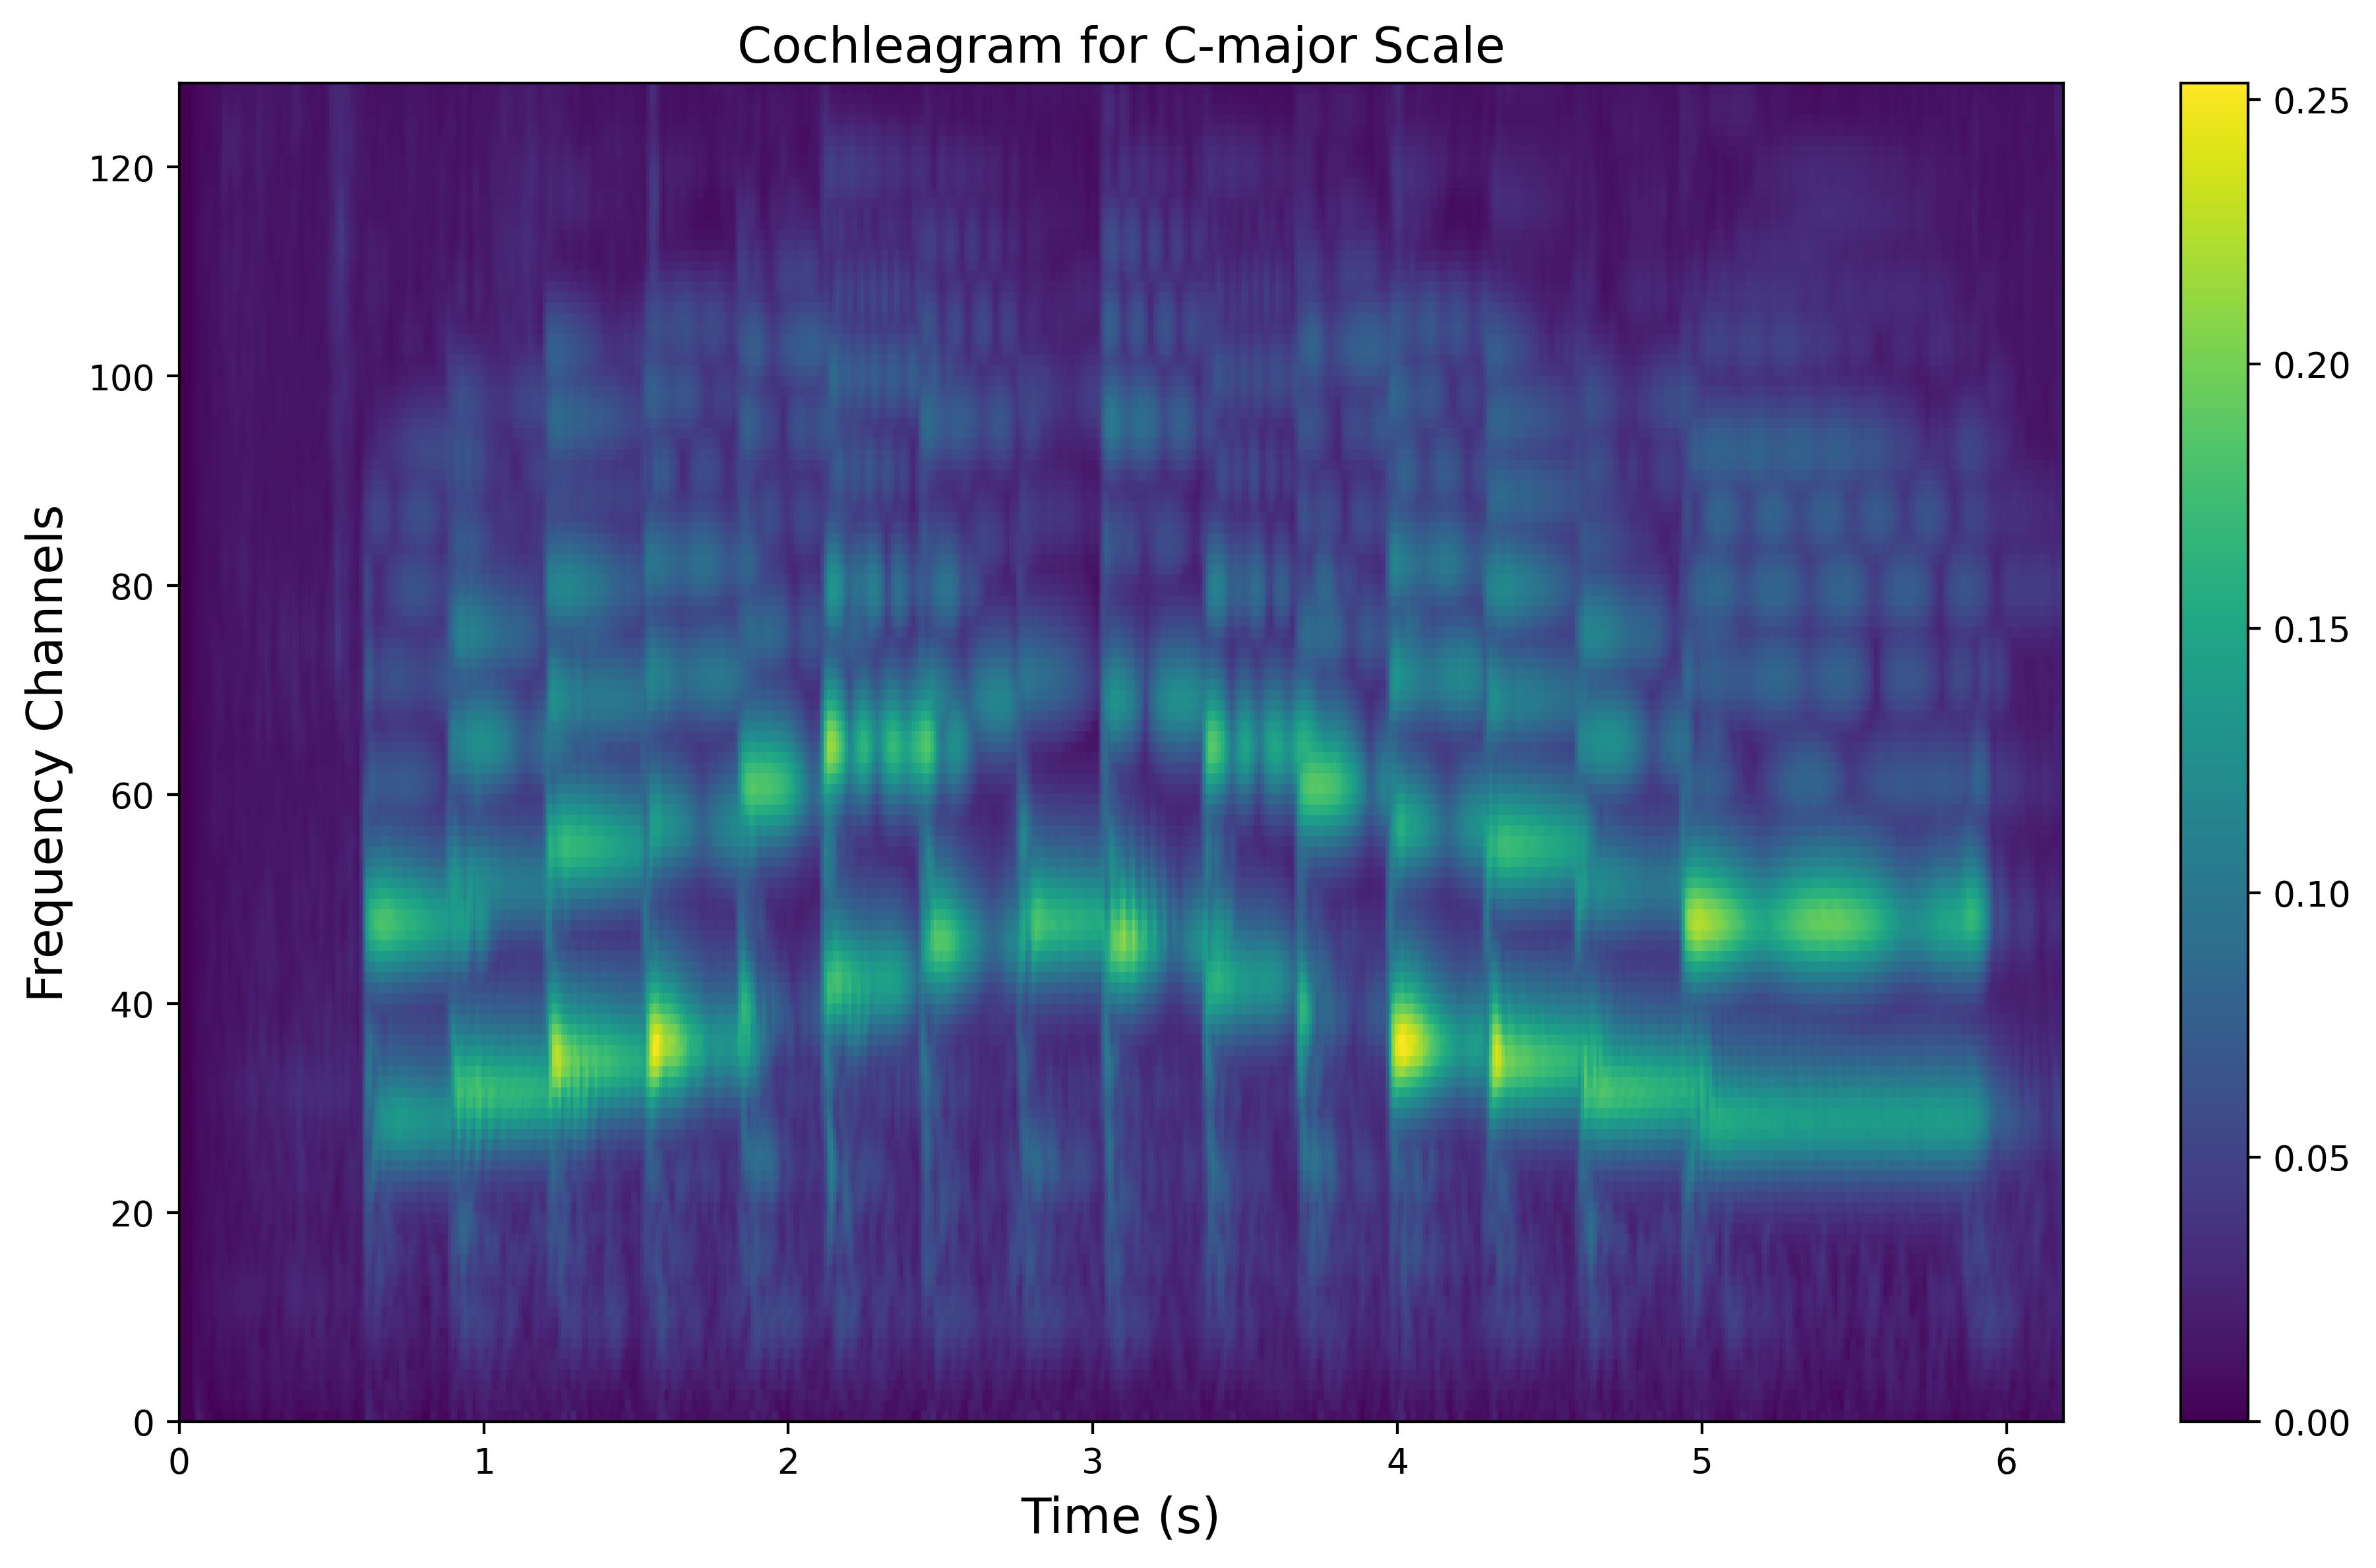
\includegraphics[width=\linewidth]{include/cochleagram_example_C-major}
		\caption{}
		\label{img:cochleagram_example_C-major}
	\end{subfigure}%
	\begin{subfigure}{0.5\textwidth}
		\centering
		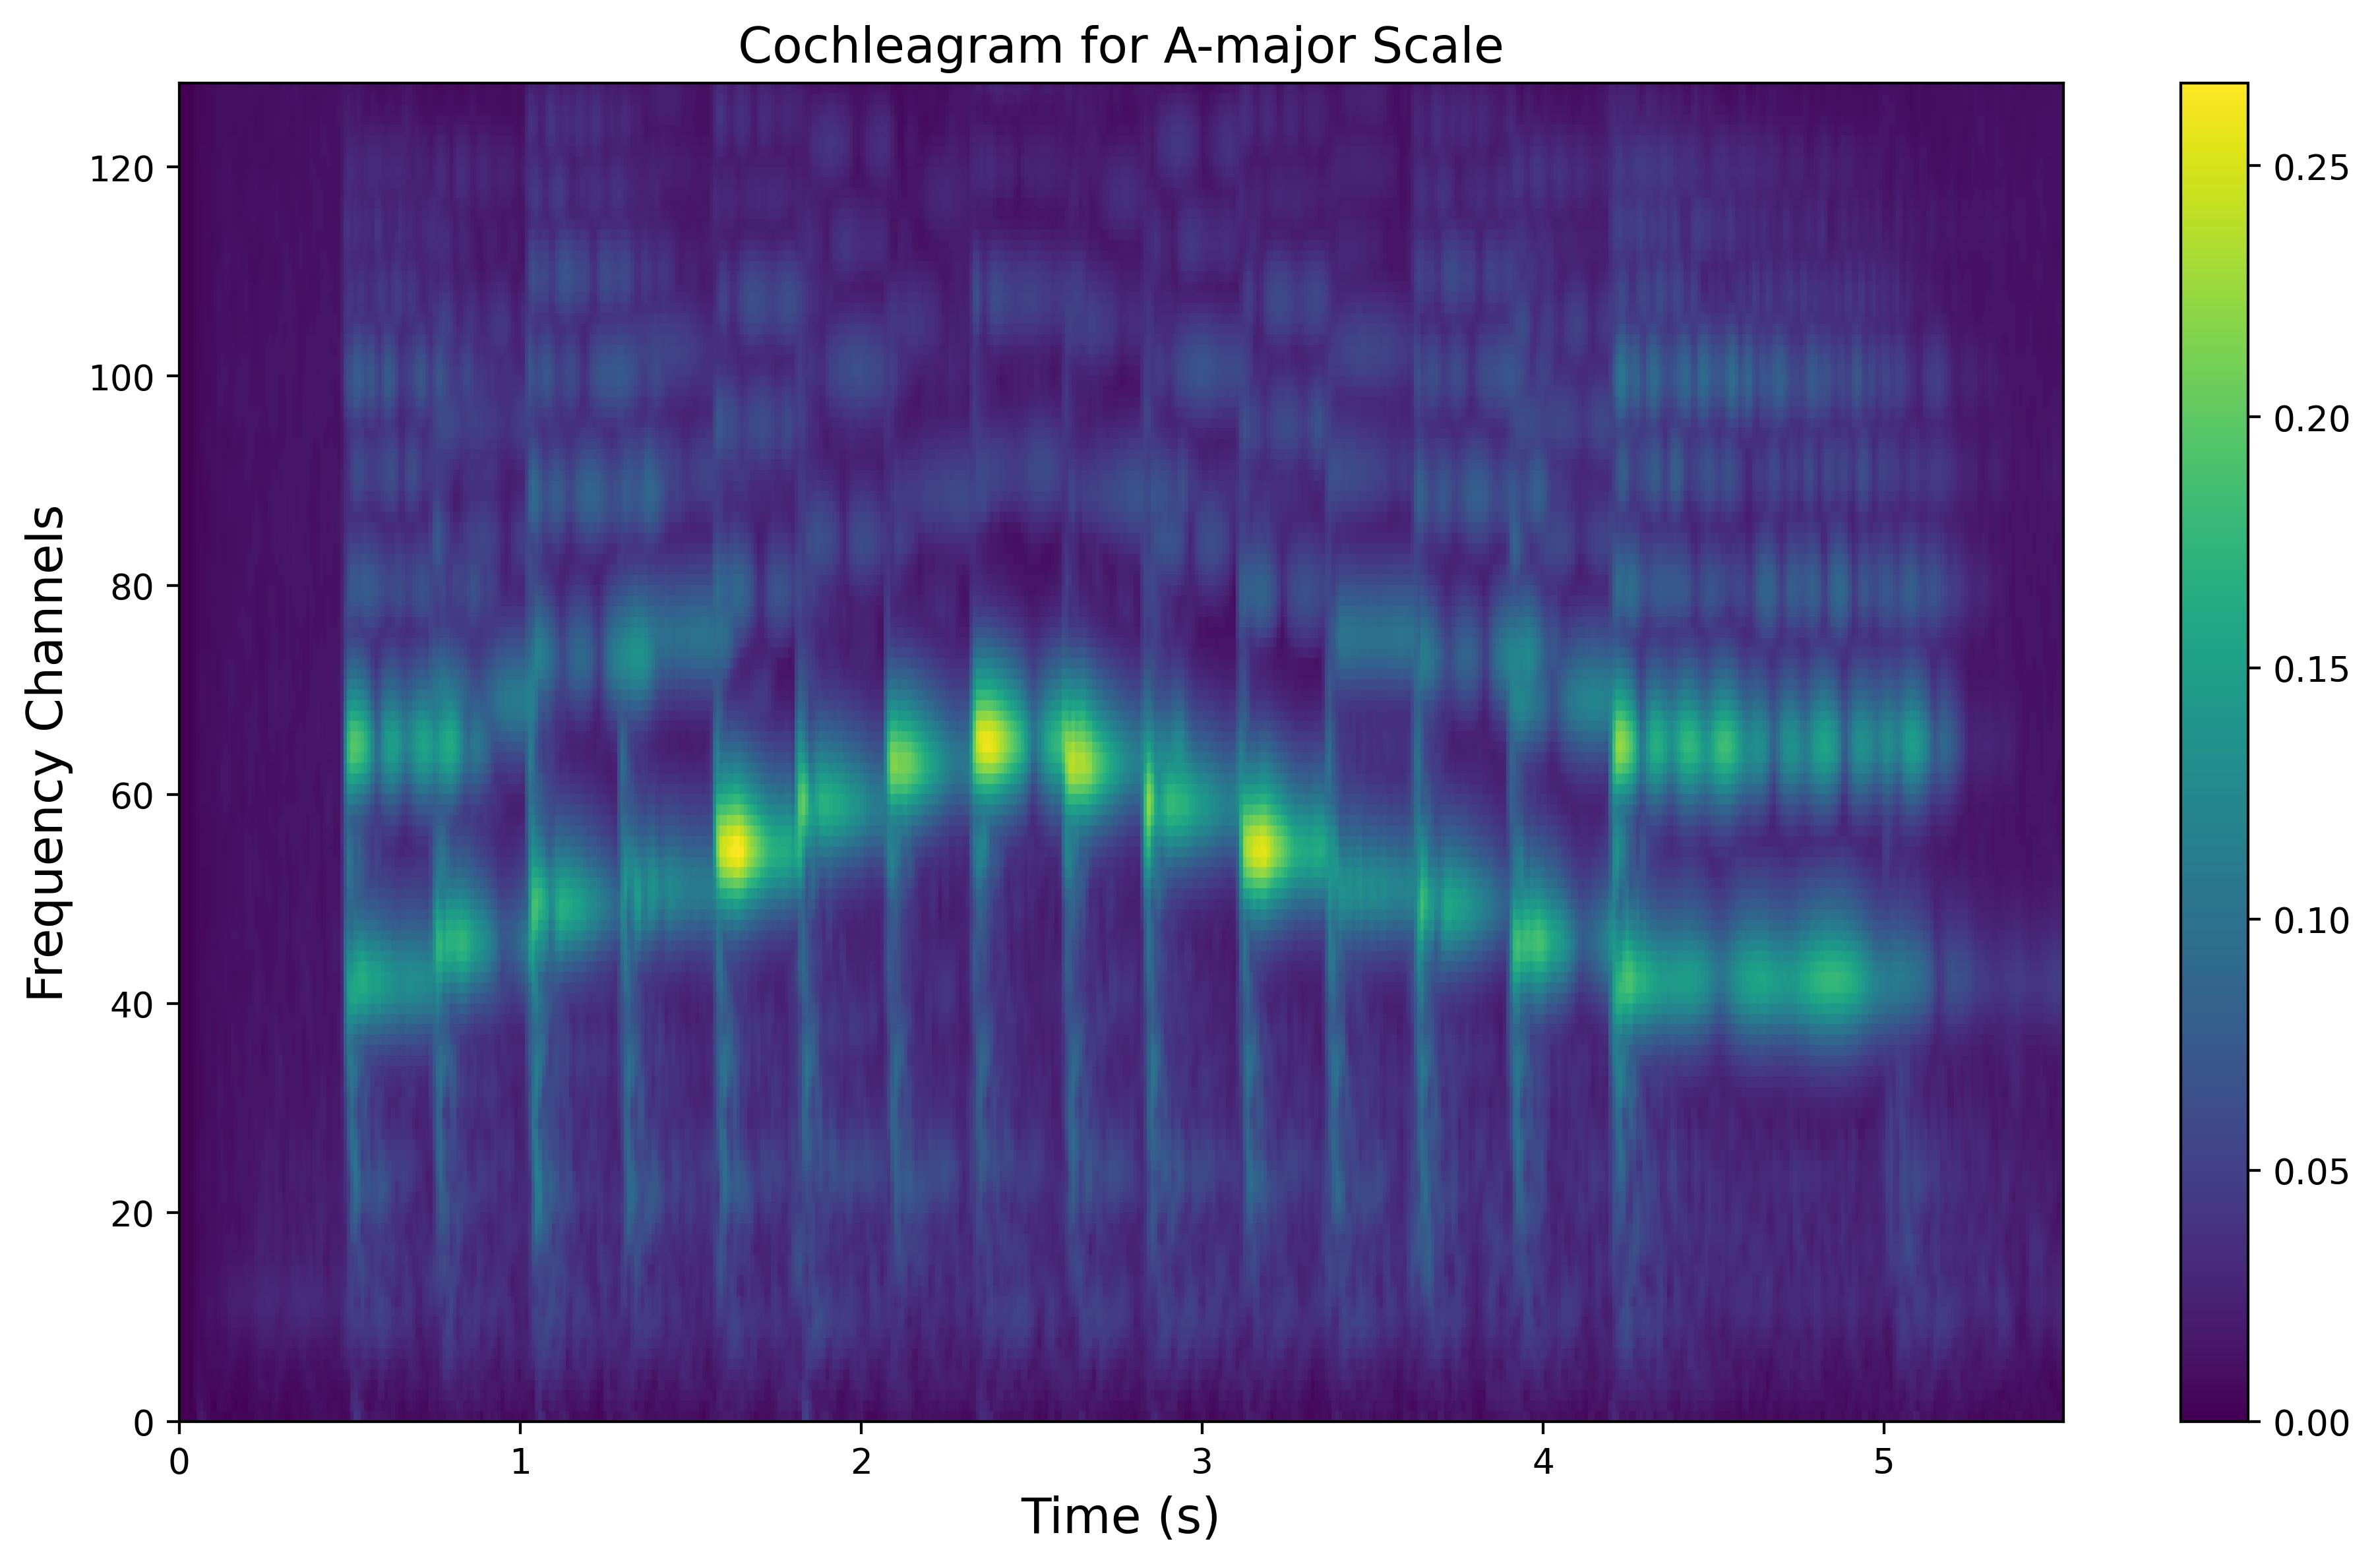
\includegraphics[width=\linewidth]{include/cochleagram_example_A-major}
		\caption{}
		\label{img:cochleagram_example_A-major}
	\end{subfigure}
	\caption[Comparison of cochleagrams for C-major and A-major scales]{Cochleagrams for C-major \textbf{(a)} and A-major \textbf{(b)} scales. The ascending and descending note progressions and the note harmonics are clearly visible in both cases, as well as the difference in fundamental frequency between the tones (all notes from A-major scale are higher).}
	\label{img:cochleagram_example}
\end{figure}

After the cochleagram was computed, is was needed to split the output into windows for further processing. A rectangular window of size 20\,ms was used as a default with an overlap of 10\,ms.

\section{Correlogram and Other Features}

For the feature extraction stage described in section \ref{subsection:casa_feature_extraction}, a correlogram was implemented using the autocorrelation function implemented in the \textit{statsmodels} package. The provided implementation could compute the ACF similarly as defined in equation \ref{equation:ACF}, however its other variant which uses Fast Fourier Transform was used for higher efficiency. The default number of lags for the autocorrelation function was chosen to be equal to the number of samples in the sampling window, i.\,e.~20\,ms times the samplerate of the input sound (48\,kHz).\\

Thus, the resulting correlogram was a three-dimensional array of floats in $[-1, 1]$ range. The first dimension was time frames, the second was frequency channels and the third was lags for the autocorrelation function.\\

Next, the summary autocorrelation function was computed to help with extracting the fundamental frequencies for separate time frames. The formula was exactly the same as in equation~\ref{equation:SACF}. Also, for demonstration purposes, cross-channel correlation was computed as defined in equation~\ref{equation:CCCF}.\\

Finally, the SACF was used to estimate the fundamental frequencies of the signals in each time frame. For this step, the "dominant" lags were firstly found, meaning equally spaced lags with the highest sum of SACF values, and then the fundamental frequency was estimated for the current time frame using the distance between two adjacent lags. The default number of "dominant" harmonics for searching was initially chosen to be 5. The resulting correlogram for time frame 150 is~shown on figure \ref{img:correlogram_example} along with all extracted features.

\begin{figure}[t]
	\centering
	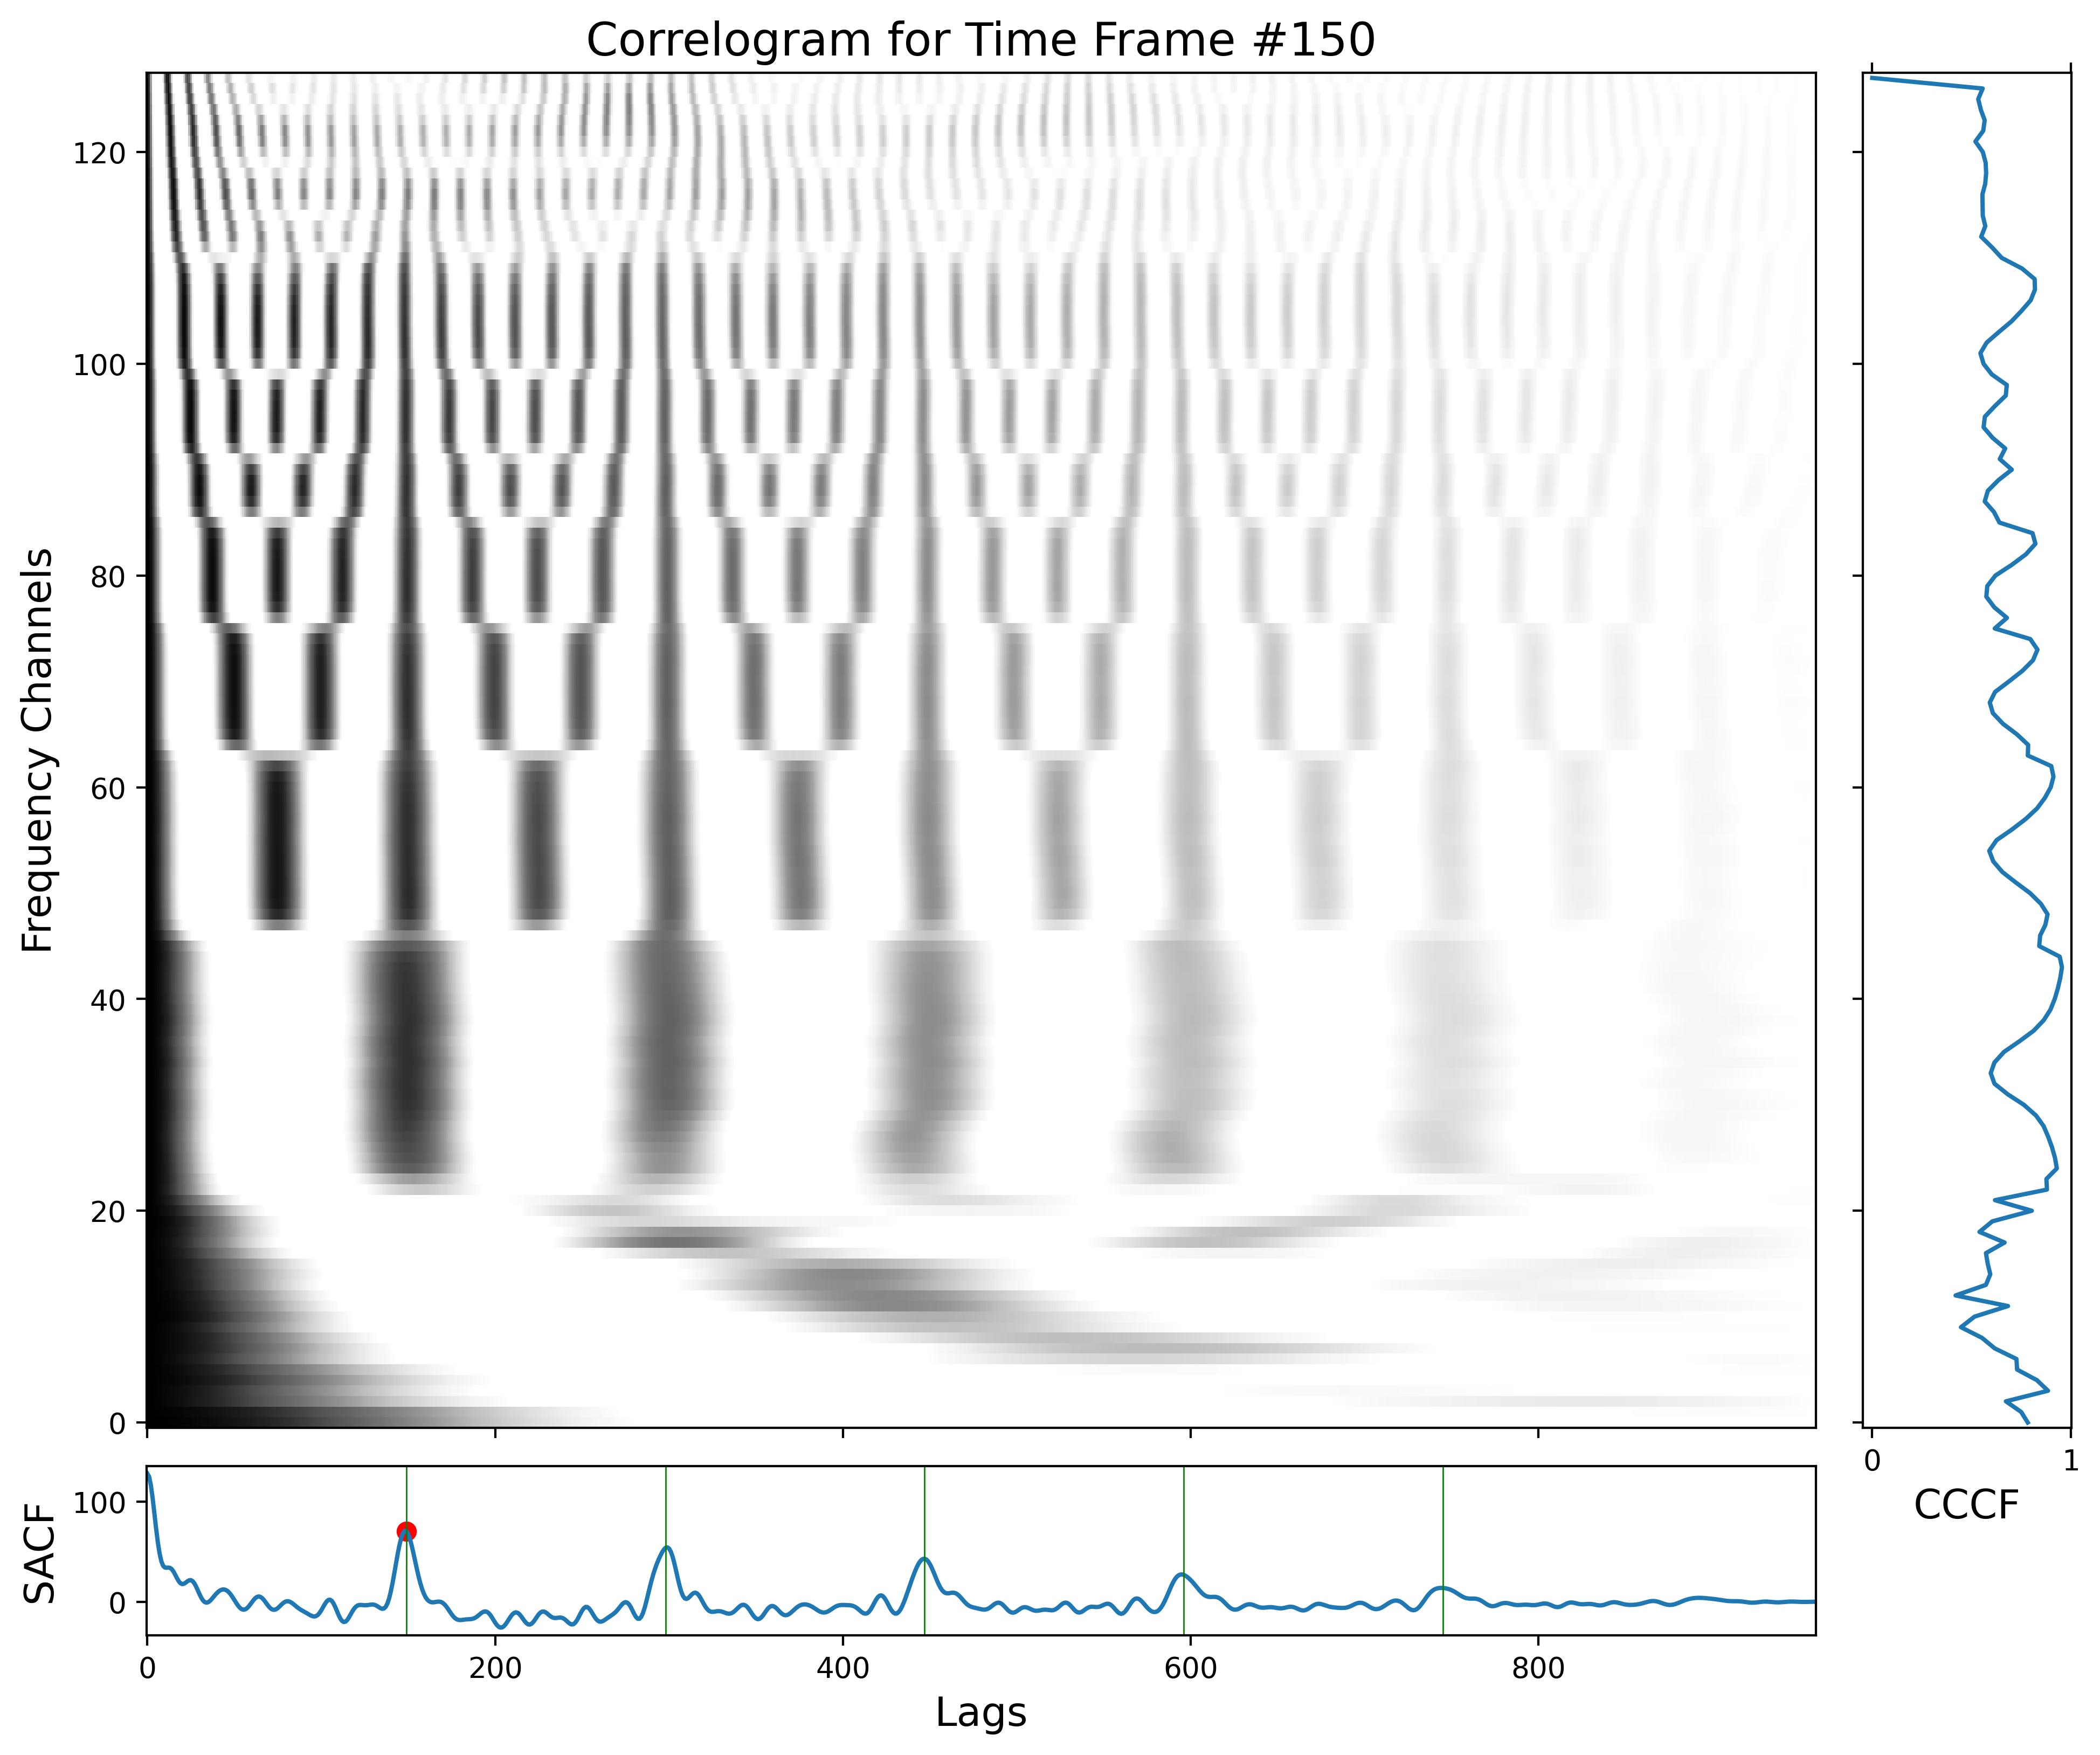
\includegraphics[width=\textwidth]{include/correlogram_example}
	\caption[An example of correlogram and the extracted features for C-major scale]{An example of a correlogram for C-major scale for time frame 150. Note that distinct frequency channels have similar repeating patterns corresponding to the repetitions observed in harmonics. The pattern starts around the frequency channel 40 and repeats twice as fast around channel 60, then three times as fast around channel 70, and so on. Cross-channel correlation is shown on the right panel, and the summary autocorrelation is shown on the bottom panel. Note the peaks on the plot for SACF that emerge when all harmonics become "synchronized" (emphasized with vertical green lines). The SACF value for the lag corresponding to the fundamental frequency is marked with a red dot.}
	\label{img:correlogram_example}
\end{figure}

\section{Masking}

The segmentation-and-grouping stage involved the task of estimating the ideal binary mask for the cochleagram computed in the first part. This step was done by combining two matrices described below.\\

The first matrix playing a big role in the resulting IBM was an "energy mask". This mask helped to emphasize the regions of the cochleagram that contained high sound energy by comparing the mean value of the samples in a T-F unit with a threshold. As a result, silent regions of the cochleagram --- like the ones that usually appear at the beginning of a recording --- were addressed and considered as ones not associated with the target sounds (the resulting binary energy mask contained zeroes for such T-F units). The default value for the threshold was chosen to be $0.05$.\pagebreak

\begin{figure}[t]
	\centering
	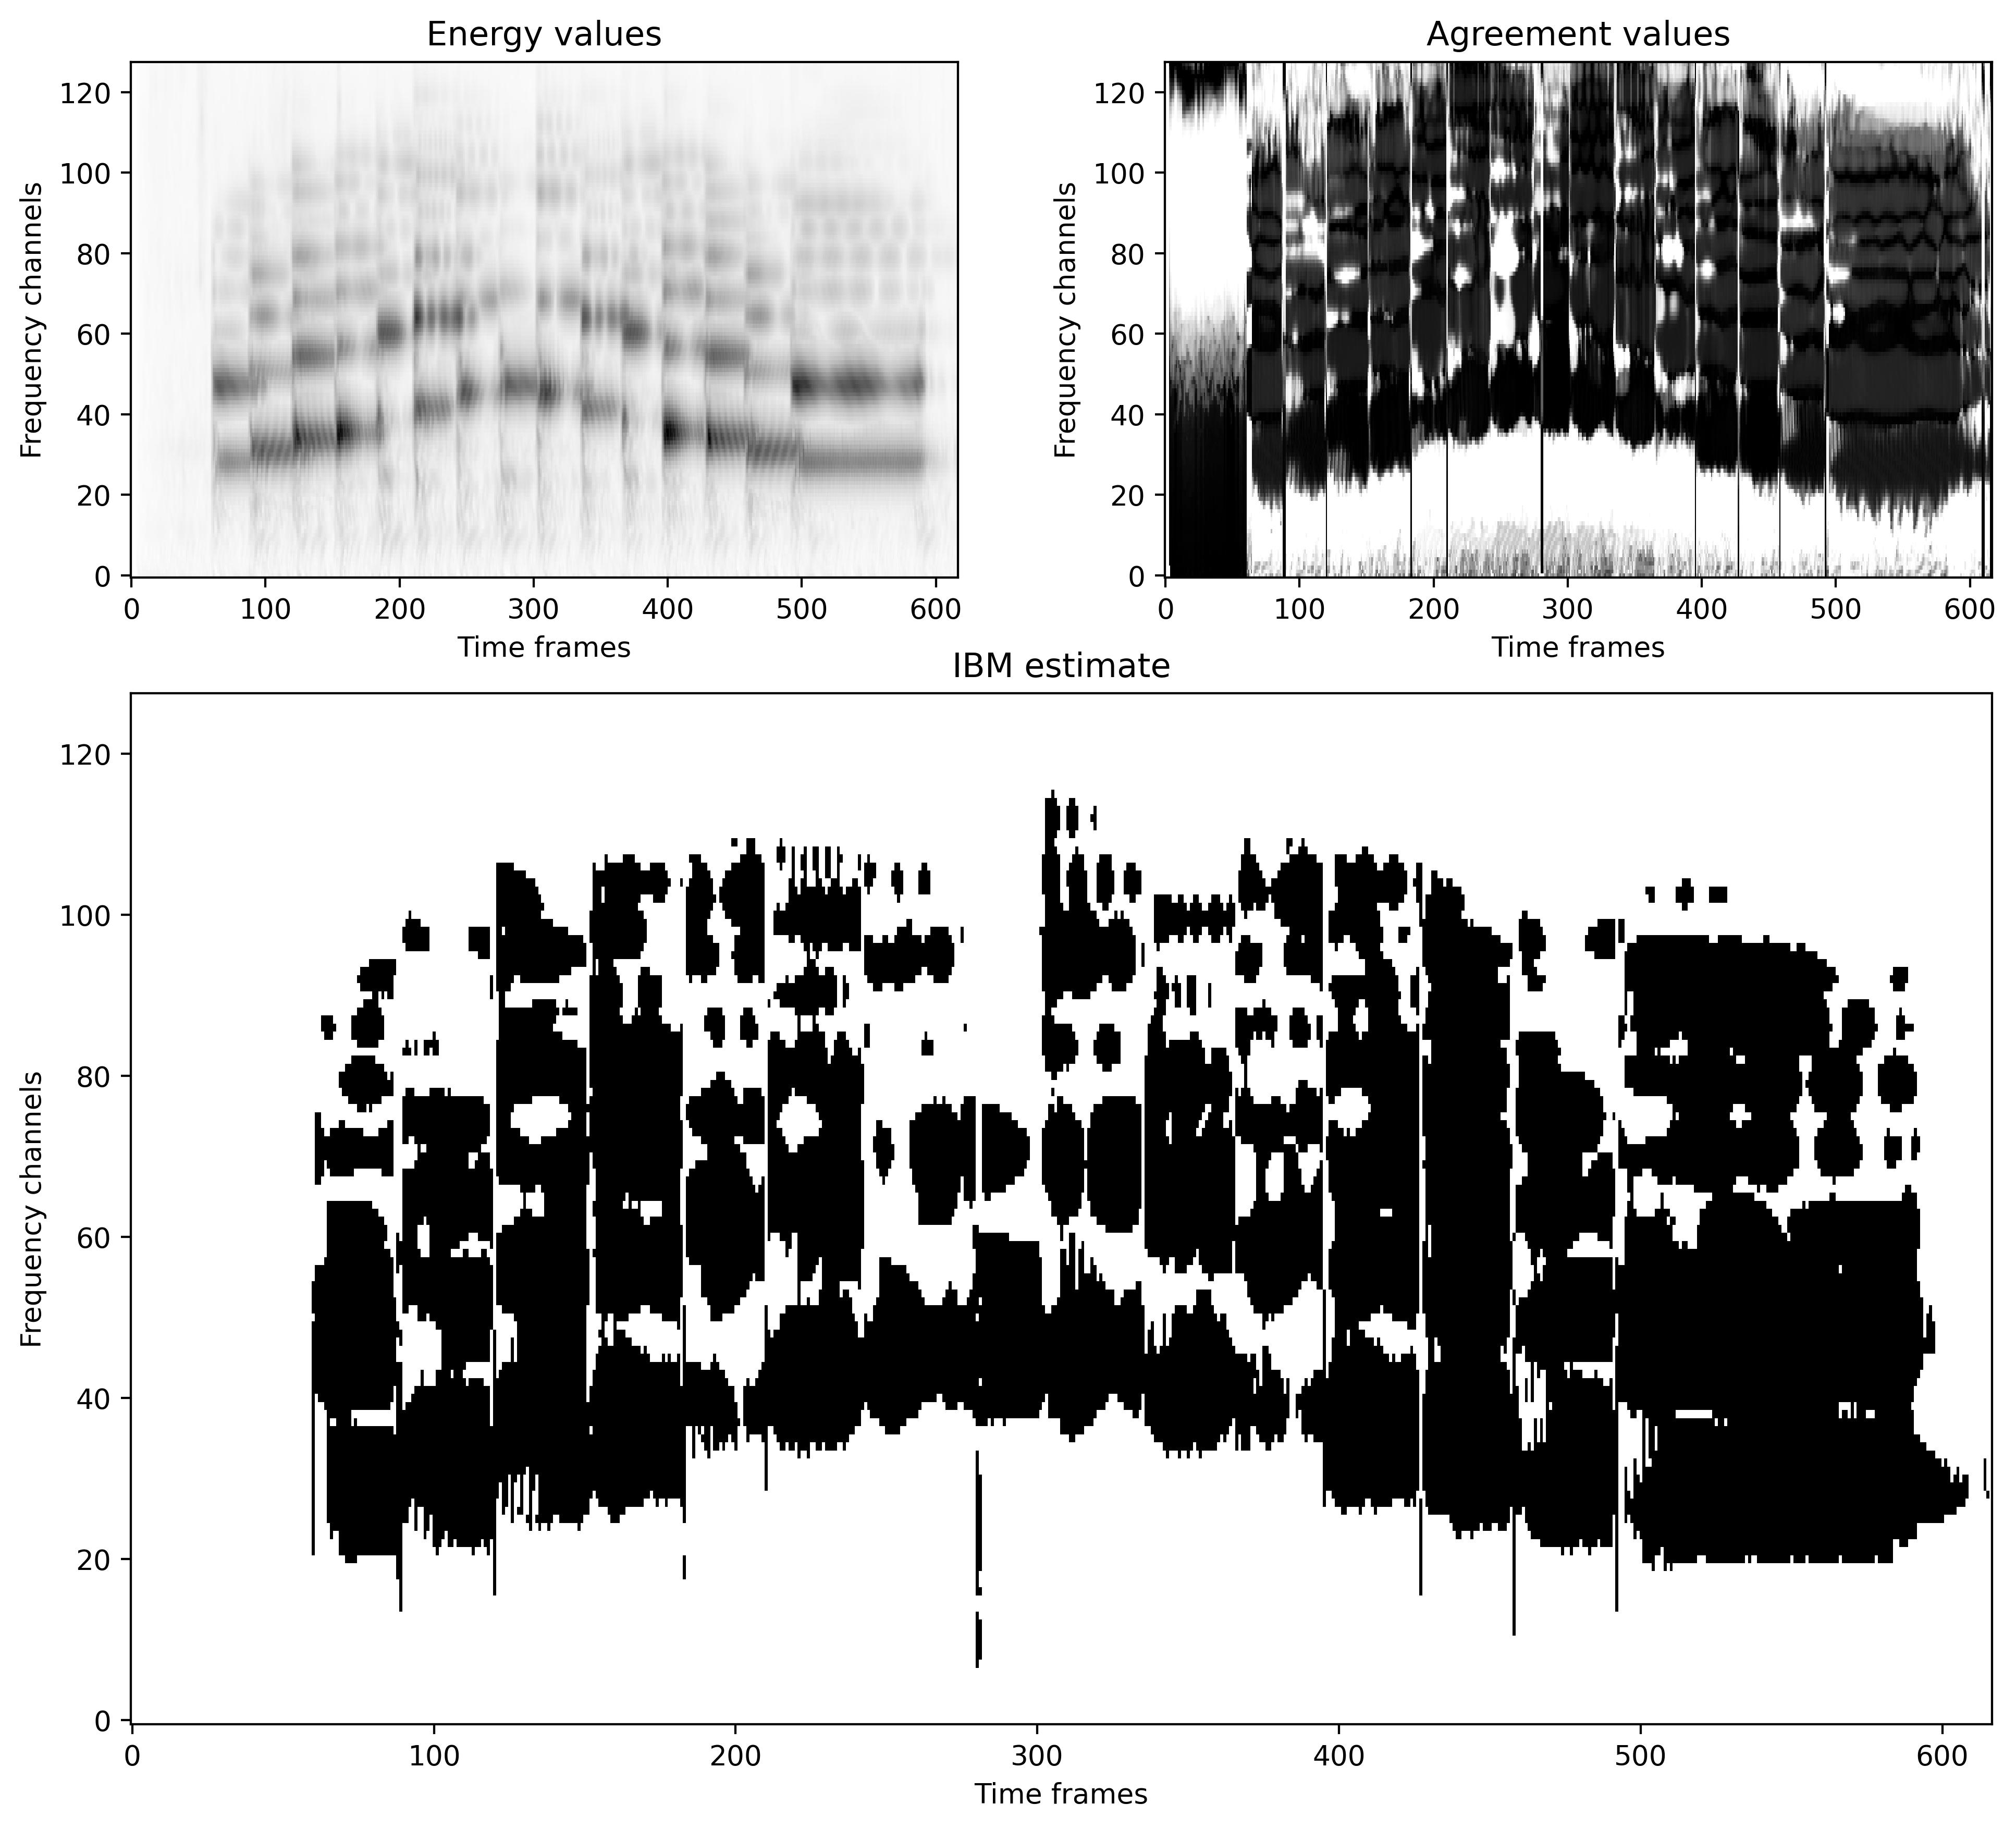
\includegraphics[width=\textwidth]{include/ibm_example}
	\caption[An example of an ideal binary mask for C-major scale]{An example of an ideal binary mask for C-major scale. The mask was estimated from combining two other masks computed by comparing sound energy and agreement values with thresholds.}
	\label{img:ibm_example}
\end{figure}

The second matrix was an "agreement values mask". This one was extracted from the correlo\-gram by taking values at the estimated "dominant" lags. These measures technically showed which frequency channels contained the harmonics of the fundamental frequency, and which did not (with some exceptions). The values were also normalized by the maximum value of the autocorrelation for the T-F unit. To make a binary decision about the measures of agreement, a threshold was used, and it was set to $0.7$ by default.\\

Finally, an ideal binary mask was estimated by combining the two above-mentioned masks using the logical-and operation. In the end, the values in the resulting IBM were set to~1 for T-F units that had mean sound energy higher than the threshold and were in agreement with the estimated fundamental frequency. An example of energy and agreement matrices and the corresponding IBM for C-major scale is shown on figure \ref{img:ibm_example}.\\

The next step was to apply the estimated mask to a cochleagram. This was done by rebuilding the cochleagram from its windowed representation and multiplying the samples in the windows by the values from the mask. The result for C-major scale is shown on figure \ref{img:masked_cochleagram_example}.\pagebreak

\begin{figure}[t]
	\centering
	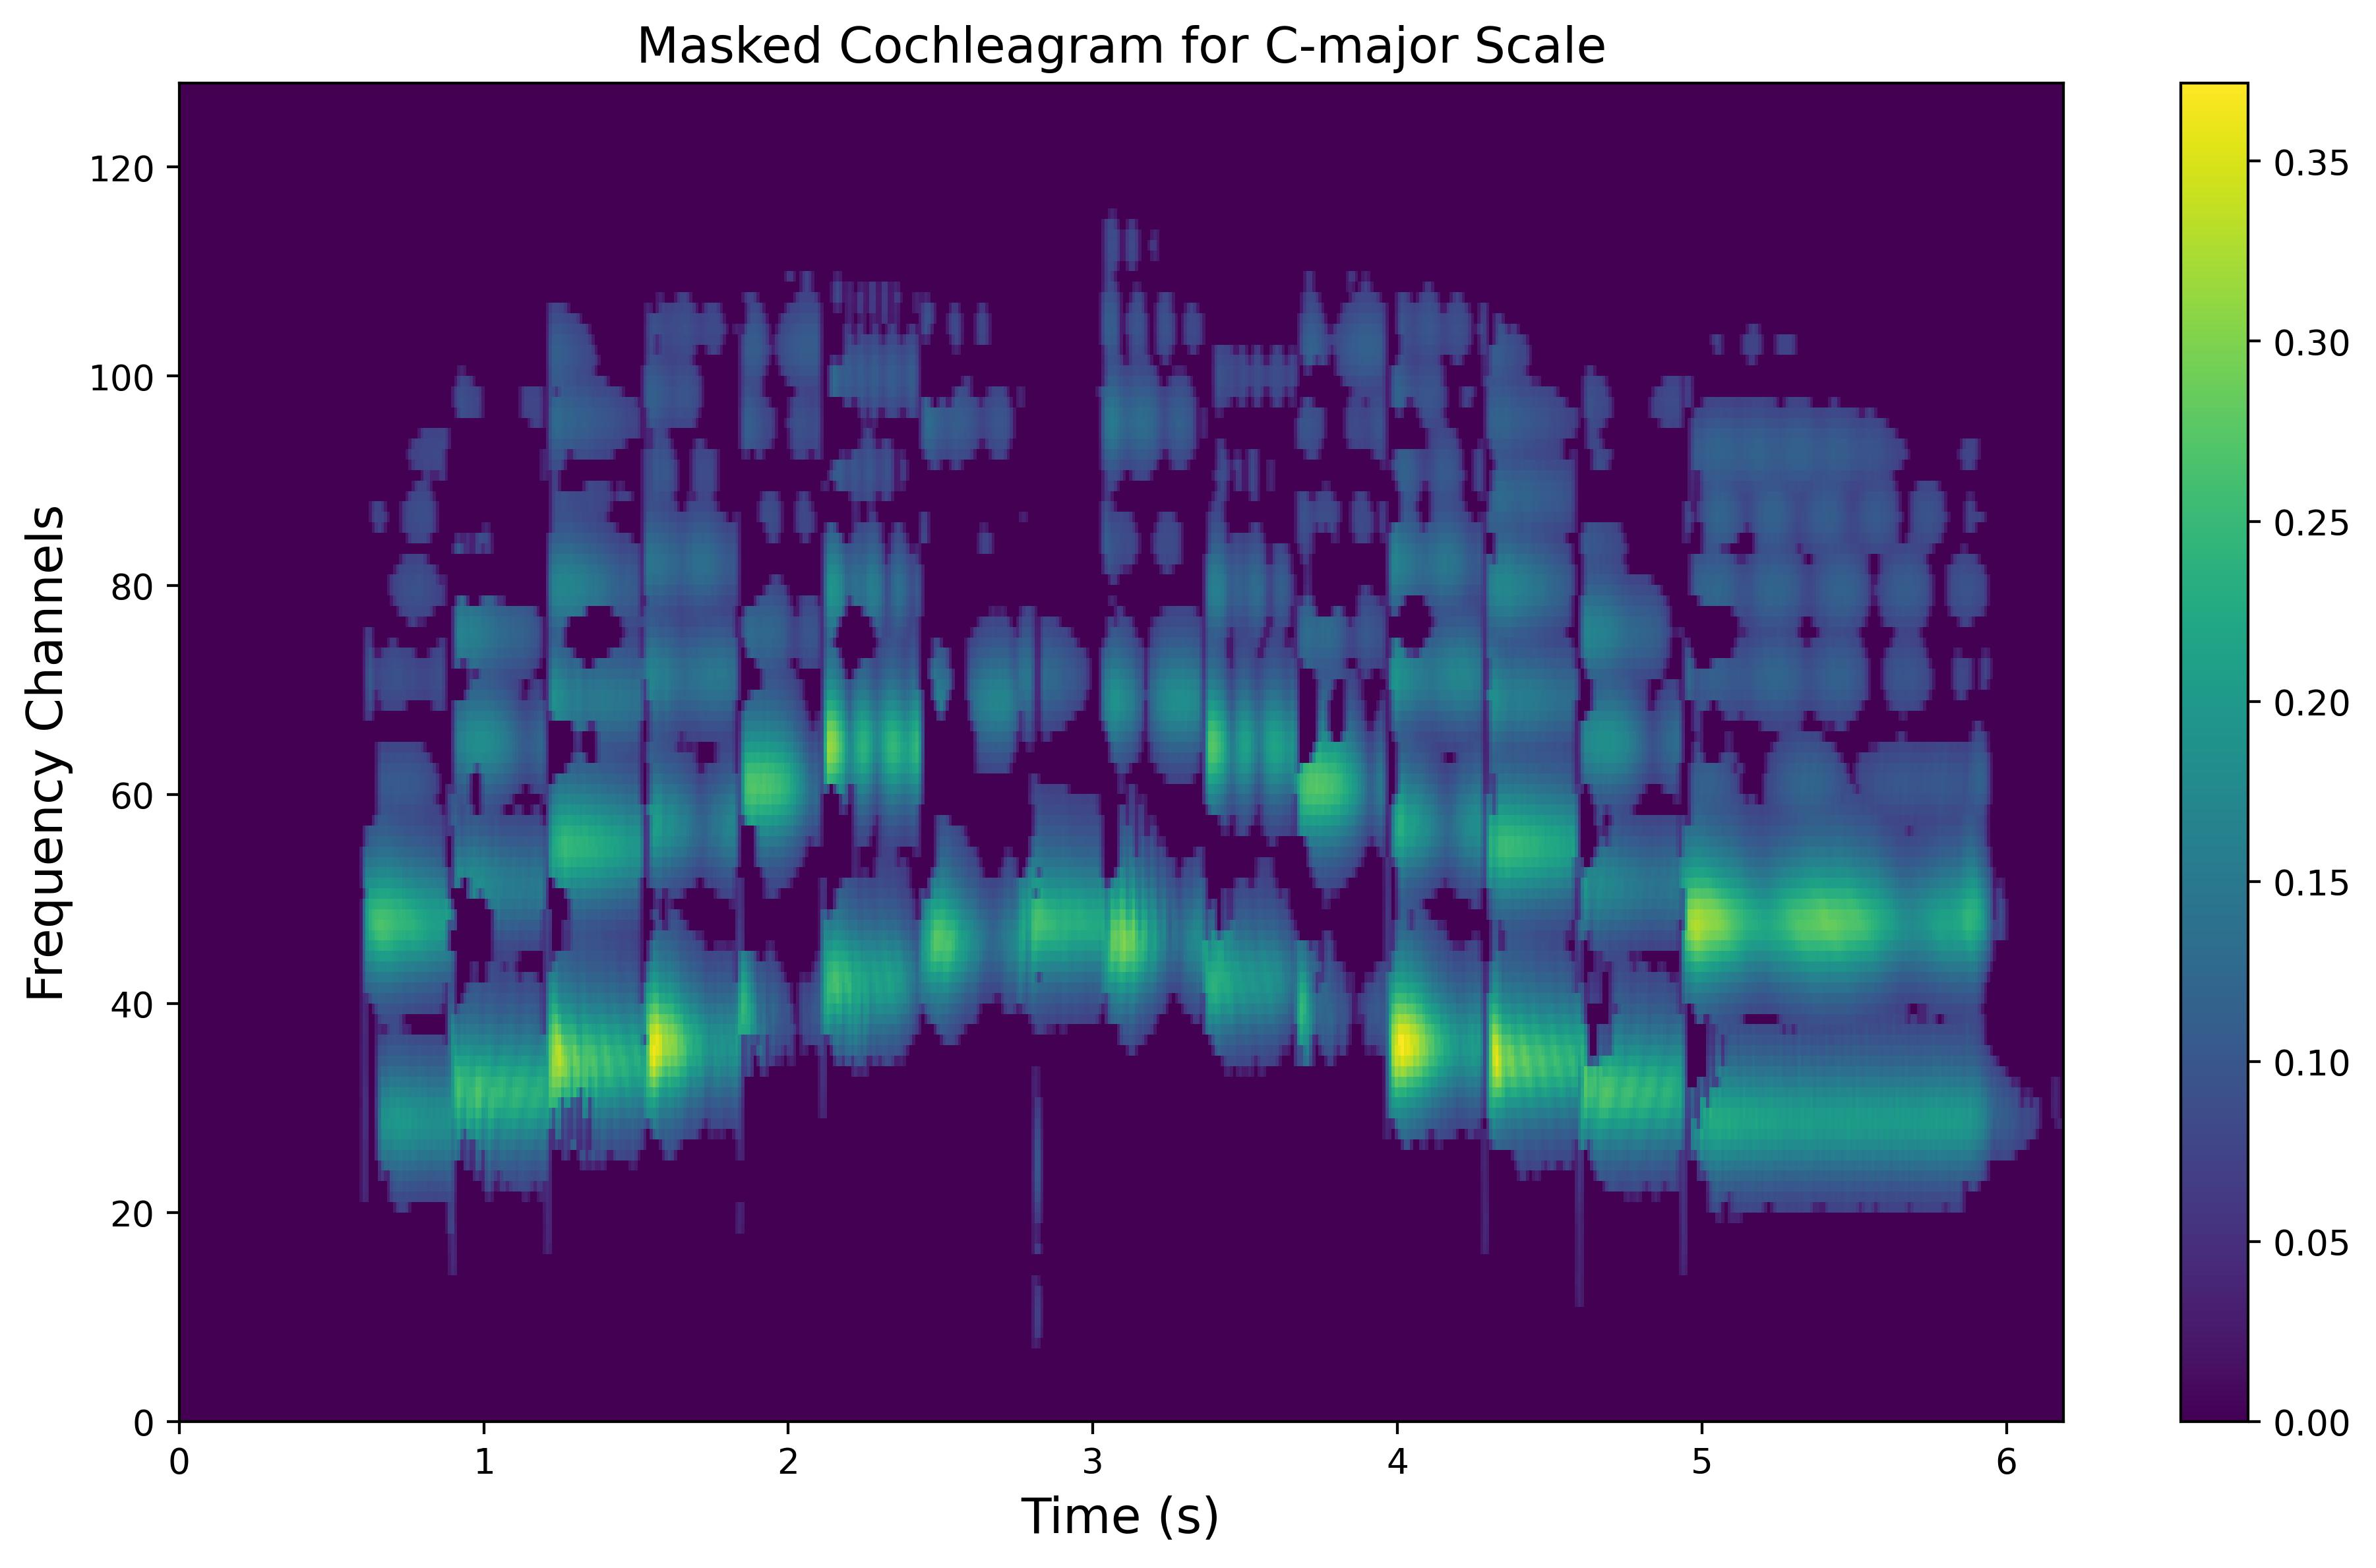
\includegraphics[width=0.85\textwidth]{include/masked_cochleagram_example}
	\caption[A masked cochleagram for C-major scale]{The cochleagram from figure \ref{img:cochleagram_example_C-major} masked by the IBM shown on figure \ref{img:ibm_example}. The main energy regions corresponding to distinct notes were kept, while the background sounds were filtered out. The ascending and descending note progressions as well as higher harmonics of the notes are also clearly visible after the masking.}
	\label{img:masked_cochleagram_example}
\end{figure}

As it can be seen from the approach chosen for estimating the IBM, Bregman's references to ASA as to a two-stage process were not addressed. The segmentation-and-grouping stage was implemented by working with all T-F units at once, without firstly segregating them into segments and then grouping the segments together based on the grouping cues. As a part of future work it is planned to give this stage more scientific attention and hopefully receive better outcomes.

\section{Chapter Summary}

This chapter discussed the CASA system implemented for this thesis. With common concepts, approaches and an architecture listed in chapter \ref{chapter:methodology}, this chapter addressed input parameters of the algorithms, described details of their implementation and any other non-standard approaches used in the model at different stages (like the method for the IBM estimation). Overall, each major stage of the architecture was given some attention: the cochleagram was implemented for the peripheral analysis stage, the correlogram was used for feature extraction, and the ideal binary masks were estimated to address mid-level representation and scene organization stages. The resynthesis stage was not implemented, as it was not needed. The next chapter will focus on how the implemented model was experimented with.


